\section{Applications} \label{applications}

Implementations of neural networks \ref{nn} (sometimes referred to as the black box) have been used for decades. The goal is to recommend visually similar images to those, which has user interacted with. Furthermore, this system can recommend advertisements which translate into revenue for the social platform. 

\begin{figure}[H]
    \centering
    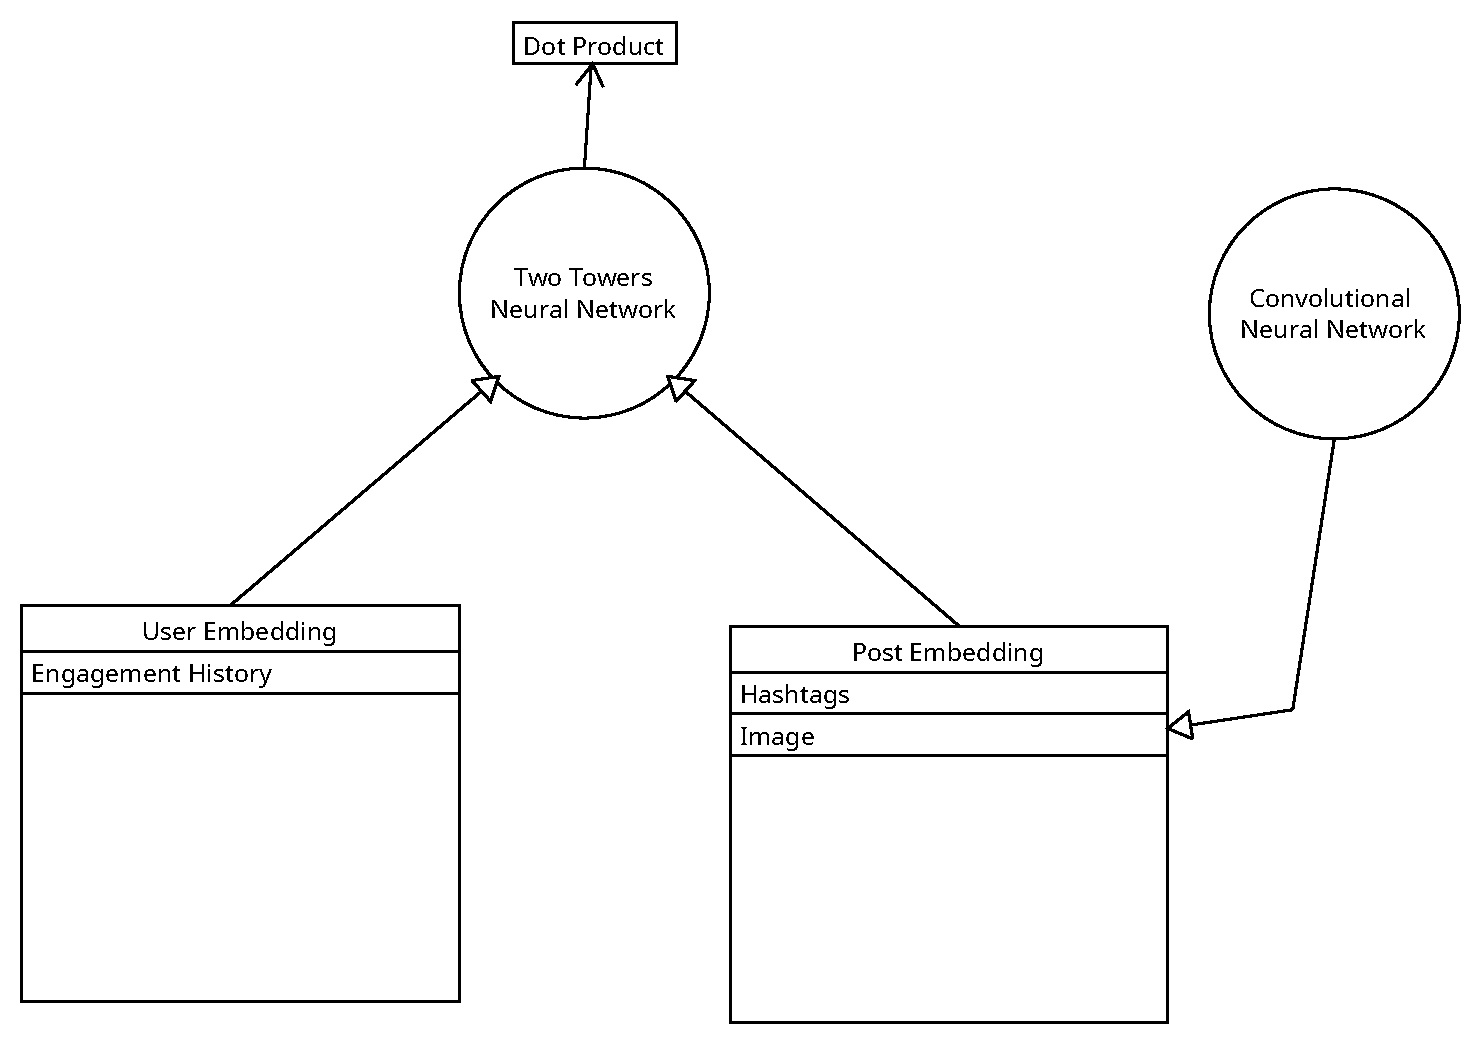
\includegraphics[width=0.7\linewidth]{Diagrams/architecture.pdf}
    \caption{Proposed architecture for content based image recommendation system}
    \label{fig:proposed-alogrithm}
\end{figure}

One of the main challenges in recommendation systems is recommending posts to a new users, who cannot be scored against existing posts. Such a problem is called ‘Cold Start' \ref{cold-start} problem. \cite{10373857} Similar problem rises for recommending new posts to users.

\subsection{Content Based Filtering}\label{applications/content-based-filtering}

This type of filtering uses machine learning to make sure people are always seeing content that is the most interesting and relevant to them. \cite{ig-new-content} The filtering is based on the user and post embedding. The user embedding contains information such as age, gender, profession and their interests collected from their behavioral data. The post embedding contains hashtags, image content representation, and the rating (likes and comments).

Content fltering techniques display item information content as feature vectors and use user profiles to recommend new items to users so that an item whose feature vector resembles the user profile vector can be suggested \cite{esvdascfacsasdicars}

Therefore it's important for the system to collect data about the user. The behavioral data includes historical feedback, like user's recent likes, comments and might include things like time spent looking at a picture or frequency of interaction and other patterns. For example, the user likes to look at motivational images in the morning and something calming in the evening.

The Image Feature Representation is acquired through Convolutional Neural Networks \ref{cnn}

\begin{comment}
    image content representation
    is this right?
    find synonym?
\end{comment}

\subsection{Collaborative Filtering}\label{applications/collaborative-filtering}

To compare similarity of two accounts, this method calculates the cosine distance or dot product of two accounts. \cite{ig-explore} In experimental comparisons, the cosine similarity function was found to perform better than the dot product function. \cite{10408929} This way, users are filtered into groups of people with the same interests. After you have engaged with content from accounts of a certain group, you will be recommended more content from similar accounts. 

\begin{comen}
    Formula for both cosine and dot products   
\end{comen}

\begin{figure}[H]
    \centering
    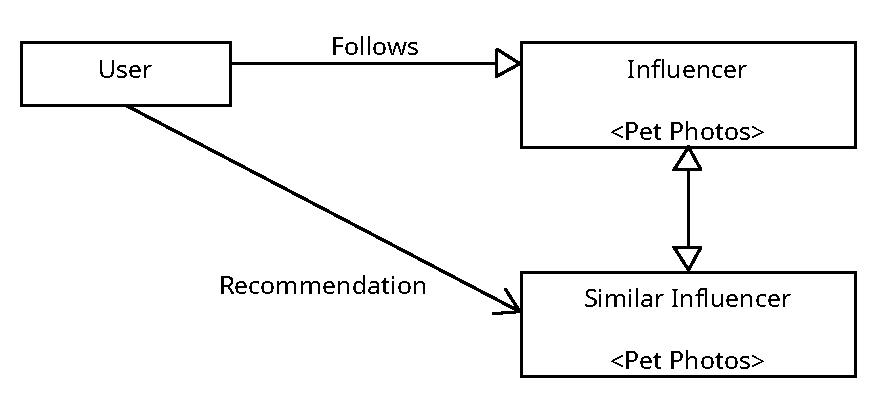
\includegraphics[width=1\linewidth]{Diagrams/collaborative-filtering.pdf}
    \caption{Example of account recommendation}
    \label{fig:collaborative-filtering-diagram}
\end{figure}
